\begin{figure*}
    \begin{subfigure}{.333\textwidth}
        \centering
        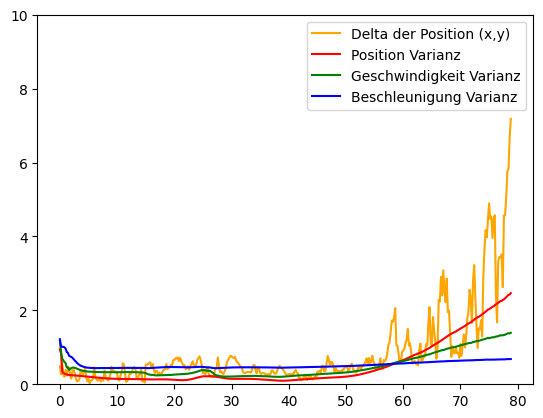
\includegraphics[width=.9\linewidth]{Ergebnisse/plots_ungenauigkeiten/richtung/richtung_dyn_acc_basic.png}
        \caption{Optimale Simulationsbedinungen}
    \end{subfigure}    
    \begin{subfigure}{.333\textwidth}
        \centering
        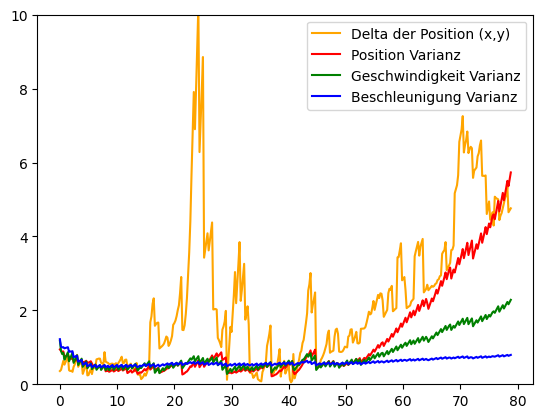
\includegraphics[width=.9\linewidth]{Ergebnisse/plots_ungenauigkeiten/richtung/richtung_dyn_acc_freq.png}
        \caption{Türme unterschiedlich frequent}
    \end{subfigure}    
    \begin{subfigure}{.333\textwidth}
        \centering
        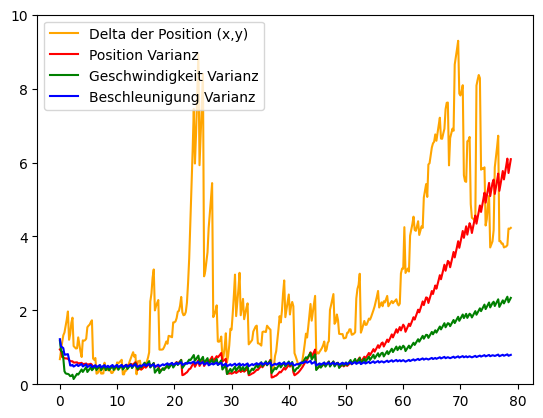
\includegraphics[width=.9\linewidth]{Ergebnisse/plots_ungenauigkeiten/richtung/richtung_dyn_acc_flag_freq.png}
        \caption{Türme unterschiedlich frequent, ausfallend}
    \end{subfigure}
    \caption{Richtungsansatz: Fehler und Varianzen bei konstanter Geschwindigkeit}
    \label{abb:richtung-da-fehler}
\end{figure*}